\chapter{النمو التكاثري والتحكم في الإزهار}\label{ch:b2:plant-flowering}

يستطيع مزارع الأقحوان أن يجعل دفيئة تزهر لعيد الميلاد
أو لعيد الفصح بتبديل الأضواء؛ وقمح الشتاء المزروع في
الربيع لا يزهر البتة، لأنه لم يبرد؛ ونبات الخرشوف الشوكي
الذي رأى ليلة واحدة أطول من طوله الحرج
يلتزم بالإزهار مهما حدث بعد ذلك. وليس للنبات تقويم،
لكن له ساعات وموازين حرارة ومقاييس ضوء، وهو يقرر مرة في
السنة، بشهادتها، أن يحوّل مرستيمًا كان يصنع الأوراق إلى
\omterm{def:b2:plant-meristems:meristem}{مرستيم} سيصنع \omterm{def:b2:angiosperm-reproduction:flower}{زهرة}. يتتبع هذا الفصل ذلك القرار
من الورقة التي تقيس الليل إلى \omterm{def:b2:plant-meristems:meristem}{المرستيم} الذي يغير برنامجه، ثم
بناء \omterm{def:b2:angiosperm-reproduction:flower}{الزهرة} بشفرة من المورّثات، ثم الانتقال
المعاكس عند الطرف الآخر من الدورة: أي \omterm{def:b2:angiosperm-reproduction:seed}{البذرة} التي لا
تنبت حتى يُقال لها إن الموسم مواتٍ.

\section{الانتقال إلى الإزهار}

\begin{definition}[الانتقال الزهري والاستحثاث الزهري]\label{def:b2:plant-flowering:transition}
\index{انتقال زهري}\index{استحثاث زهري}\index{مرستيم نوري}
\omterm{def:b2:plant-meristems:meristem}{المرستيم} القمي الخضري للفرع يصنع أوراقًا في إبط كل منها برعم،
بلا نهاية. وعند \emph{الانتقال الزهري} يصير
\emph{مرستيمًا نوريًا}، يصنع قنابات وفي آباطها
\emph{مرستيمات زهرية}، كل منها محدد: إذ
يصنع سبلات وبتلات وسدى وكرابل ثم يتوقف. ويطلق التغيرَ
\emph{الاستحثاث الزهري} --- أي إشارة، آتية من
الأوراق أو ناشئة في فيزيولوجيا النبات نفسها، تبدّل مورّثات
هوية \omterm{def:b2:plant-meristems:meristem}{المرستيم}. والحوليات تزهر مرة وتموت؛ أما
المعمّرات فتزهر كل سنة من بعض المرستيمات وتبقي الأخرى
خضرية. والتوقيت يقرر هل يلقى \omterm{def:b2:plant-life-cycles:heterospory}{اللقاح} لقاحًا، وهل تنضج
البذور قبل الصقيع، وهل تتفتح \omterm{def:b2:angiosperm-reproduction:flower}{الزهرة} حين يطير ملقّحها:
فهو تحت انتخاب شديد، وقد طوّرت النباتات طرقًا عدة
لقراءة الموسم.
\end{definition}

\begin{proposition}[الدورية الضوئية: النبات يقيس الليل]\label{prop:b2:plant-flowering:photoperiod}
\index{دورية ضوئية}\index{نبات قصير النهار}\index{نبات طويل النهار}\index{فيتوكروم}
كثير من النباتات يزهر استجابةً لطول النهار. فالنباتات
\emph{القصيرة النهار} (الأقحوان، وفول الصويا، والأرز، والخرشوف الشوكي) تزهر حين
يكون النهار أقصر من طول حرج --- في الخريف أو الربيع؛
والنباتات \emph{الطويلة النهار} (السبانخ، والقمح، والنفل، و\emph{Arabidopsis})
تزهر حين يكون أطول --- في مطلع الصيف؛ والنباتات \emph{المحايدة
النهار} (البندورة، والذرة) تزهر حين تكبر بما يكفي. والذي يقيسه النبات
هو في الواقع طول \emph{الليل} غير المنقطع: \omterm{prop:b2:plant-flowering:photoperiod}{فالنبات
القصير النهار} نبات طويل الليل، وومضة ضوء في
منتصف ليلة طويلة تلغي أثرها، في حين لا تلغيه فترة
ظلام في نهار طويل. والقياس يجري في
\emph{الأوراق}، بالصباغ \emph{الفيتوكروم} --- وهو بروتين
يتبدل بين صورة ماصة للأحمر وصورة ماصة للأحمر البعيد
مع كل فوتون يلتقطه، فتسجل حالته الضوء
--- مقروءًا في مقابل \emph{ساعة يومية} داخلية مدتها نحو
أربع وعشرين ساعة: فيُطلق الإزهار حين يتزامن الضوء مع
طور معين من الساعة، وهذا لا يقع إلا عند طول النهار
الصحيح.
\end{proposition}
\begin{proof}[شواهد]
وجد غارنر وألارد (1920) أن تبغًا طافرًا لم يزهر إلا
في أيام الدفيئة الشتوية القصيرة، وأن فول الصويا المزروع على
فترات خلال الصيف أزهر كله معًا في أيلول:
فطول النهار، لا العمر ولا الحرارة، هو الذي ضبط التاريخ. وبيّن هامنر وبونر
(1938) بالخرشوف الشوكي أن ليلة طويلة واحدة تكفي، وأن
دقيقة من الضوء في منتصف الليل تلغي الأثر،
وأن تقصير النهار دون تغيير الليل لا
يستحث. ووجد بورثويك وهندريكس (1952) أن أفعل
الضوء هو الأحمر وأن الأحمر البعيد المعطى بعد الأحمر مباشرة
يلغيه --- وهي بصمة الفيتوكروم الذي عُزل
سنة 1959. وتطعيم ورقة واحدة مستحَثة على نبات غير مستحَث جعل
النبات كله يزهر: فالورقة تصدّر إشارة.
\end{proof}

\begin{omfigure}
\begin{tikzpicture}[every node/.style={font=\scriptsize}]
  \foreach \y/\lab/\res in {3.6/{نهار طويل، ليل قصير}/{لا زهر}, 2.7/{نهار قصير، ليل طويل}/{تزهر}, 1.8/{ليل طويل تقطعه ومضة ضوء}/{لا زهر}, 0.9/{نهار طويل يقطعه ظلام}/{لا زهر}} {
    \node[anchor=east, align=right] at (-0.2,\y) {\lab};
    \node[anchor=west, omThm] at (8.6,\y) {\res};
  }
  % bars: 24 h = 8 cm; light yellow, dark grey
  \fill[omExo!30] (0,3.4) rectangle (8,3.8); \fill[yellow!50!orange!40] (0,3.4) rectangle (5.4,3.8);
  \fill[omExo!30] (0,2.5) rectangle (8,2.9); \fill[yellow!50!orange!40] (0,2.5) rectangle (3.0,2.9);
  \fill[omExo!30] (0,1.6) rectangle (8,2.0); \fill[yellow!50!orange!40] (0,1.6) rectangle (3.0,2.0); \fill[yellow!50!orange!40] (5.4,1.6) rectangle (5.55,2.0);
  \fill[omExo!30] (0,0.7) rectangle (8,1.1); \fill[yellow!50!orange!40] (0,0.7) rectangle (5.4,1.1); \fill[omExo!30] (2.6,0.7) rectangle (2.9,1.1);
  \draw[thick, ->] (0,0.3) -- (8.2,0.3); \foreach \x/\l in {0/0,2/6,4/12,6/18,8/24} \draw (\x,0.35) -- (\x,0.25) node[below] {\l};
  \node[below] at (4,-0.05) {الساعات};
  \draw[dashed, omDef] (5.4,0.3) -- (5.4,4.0); \node[omDef, above] at (5.4,4.0) {طول الليل الحرج};
\end{tikzpicture}

{\small خرشوف هامنر وبونر الشوكي، وهو \omterm{prop:b2:plant-flowering:photoperiod}{نبات قصير النهار}. يزهر
بعد ليلة أطول من الطول الحرج؛ ودقيقة من الضوء في
منتصف الليل تلغي الاستحثاث، ولا تلغيه فترة ظلام
في النهار. فالنبات يقيس الليل.}
\end{omfigure}

\begin{definition}[الفلوريجين]\label{def:b2:plant-flowering:florigen}
\index{فلوريجين}\index{FLOWERING LOCUS T}
الإشارة التي تصدّرها الورقة سُمّيت \emph{الفلوريجين} سنة 1937 و
عُرفت بعد سبعين سنة بروتينًا صغيرًا، هو ناتج
المورّثة \emph{FLOWERING LOCUS T} (FT). ففي الورقة، تشعل الساعة و
الفيتوكروم معًا المورّثة FT حين يكون طول النهار مناسبًا
(وفي \emph{Arabidopsis}، وهو \omterm{prop:b2:plant-flowering:photoperiod}{نبات طويل النهار}، حين يتزامن الضوء مع
ذروة المنشّط CONSTANS المضبوط بالساعة في العصر)؛
ثم يدخل بروتين FT اللحاء، ويسافر مع تيار السكر إلى
قمة الفرع، ويشعل هناك، مع بروتين شريك، المورّثات
التي تحوّل \omterm{def:b2:plant-meristems:meristem}{المرستيم}. والبروتين نفسه هو فلوريجين
الأرز، وهو \omterm{prop:b2:plant-flowering:photoperiod}{نبات قصير النهار}، تصله الساعة فيه على النحو
المعاكس. وتجارب التطعيم، ونقل البروتين في
اللحاء، وإزهار نباتات يُعبَّر فيها عن FT من محرّض نوعي
الورقة: كلها متفقة: \omterm{def:b2:angiosperm-reproduction:flower}{فالزهرة} تُقرَّر في
الورقة وتُنفَّذ في البرعم.
\end{definition}

\begin{omfigure}
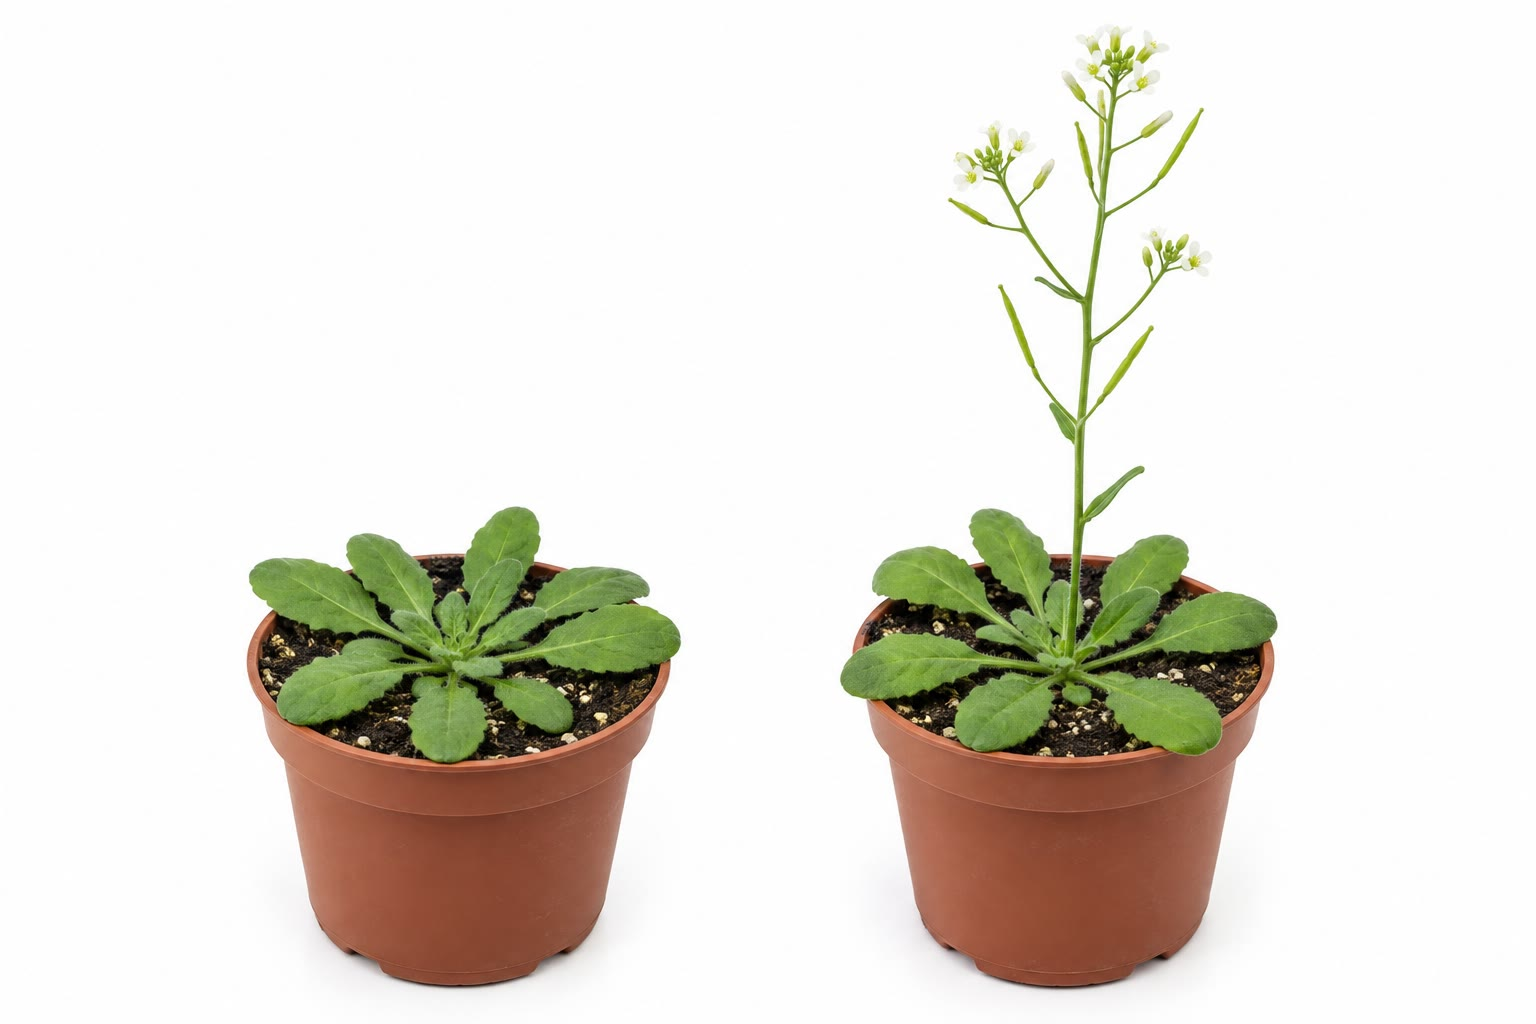
\includegraphics[width=0.58\linewidth]{images/book4/ai/b4-14-arabidopsis-daylength.jpg}

{\small \emph{Arabidopsis}، وهو \omterm{prop:b2:plant-flowering:photoperiod}{نبات طويل النهار}: في الأيام القصيرة
وريدة من الأوراق؛ وإذا نُقل إلى أيام طويلة، شرع وأزهر في غضون
أسابيع.}
\end{omfigure}

\begin{proposition}[الإرباع: النبات يعدّ البرد]\label{prop:b2:plant-flowering:vernalisation}
\index{إرباع}\index{FLOWERING LOCUS C}
الحبوب الشتوية، والثنائيات الحول (الجزر، والملفوف، وقفاز الثعلب) وكثير من
معمّرات المناخات الباردة لا تزهر حتى تكون قد
مرت بأسابيع من البرد --- وهو \emph{الإرباع} --- الذي
يضمن أن النبات المنبت في الخريف ينتظر الربيع بدل أن
يزهر في الصقيع. والبرد يستشعره \omterm{def:b2:plant-meristems:meristem}{المرستيم}
نفسه لا الأوراق؛ ولا يمكن تعويضه بأي معالجة
أخرى؛ ويُذكَر أثره بقية نمو النبات،
عبر مئات الانقسامات الخلوية، لا عبر \omterm{def:b2:meiosis-heredity:meiosis}{التقسم المنصّف}
--- فكل \omterm{def:b2:angiosperm-reproduction:seed}{بذرة} تبدأ غير مرباعة. وفي \emph{Arabidopsis}
تكون الذاكرة مورّثة، هي \emph{\omterm{prop:b2:plant-flowering:vernalisation}{FLOWERING LOCUS C}} (FLC)، يكبت ناتجها
الإزهار: فتسكتها أسابيع من البرد تدريجيًا بتغطية
صبغينها بعلامات كابتة، ويُنسخ الإسكات عند كل انقسام،
ويُمحى في الجنين. فالنبات إذن \emph{يكامل} البرد عبر الزمن --- فأيام
باردة قليلة لا تُحسب --- والطافر الذي يفتقر إلى FLC لا يحتاج شتاءً.
\end{proposition}

\begin{theorem}[لماذا تحمي المكاملة من ربيع كاذب]\label{thm:b2:plant-flowering:integration}
لنفترض أن كابتًا يُسكت بمعدل ثابت $\alpha$ في اليوم
البارد الواحد، فيكون الكسر الباقي فعالًا بعد $n$ يومًا باردًا
$f_n = e^{-\alpha n}$، وأن الإزهار يُسمح به حين $f < f_c$.
فعدد الأيام الباردة اللازمة هو $n_c = \ln(1/f_c)/\alpha$، و
--- لأن الإسكات ثابت --- لا يلزم أن تكون الأيام الباردة
متتالية: وإنما المهم مجموعها. فالنبات الذي عنده $n_c = 40$
يومًا لا يخدعه ذوبان أسبوعين في كانون الثاني ولا موجة
برد في تشرين الأول؛ أما النبات الذي يستشعر الحرارة الحالية وحدها
فكان ليزهر في أول أسبوع دافئ. والمكاملة نفسها، مع
عتبة، هي كيف يقرأ النبات طول النهار المتراكم قبل
الالتزام؛ وكلاهما مثال على جملة تستجيب
إلى \emph{تكامل} إشارة لا لقيمتها اللحظية.
\end{theorem}
\begin{proof}
إذا أسكت كل يوم بارد كسرًا $\alpha$ من النسخ الفعالة
الباقية (أو من الصبغين الذي لم يُعلَّم بعد)، خضع الكسر
الفعال للعلاقة $f_{n+1} = (1 - \alpha)f_n \approx e^{-\alpha}f_n$،
ومنه $f_n = e^{-\alpha n}$ حيث $n$ عدد الأيام الباردة؛ و
المتراجحة $e^{-\alpha n} < f_c$ تعطي $n > \ln(1/f_c)/\alpha$.
أما الأيام غير الباردة فلا تضيف ولا تطرح، إذ إن العلامات
ثابتة، فلا يهم إلا المجموع.
\end{proof}

\section{بناء الزهرة: نموذج ABC}

\begin{proposition}[نموذج ABC]\label{prop:b2:plant-flowering:abc}
\index{نموذج ABC}\index{مورّثة مثلية!زهرية}
يضع \omterm{def:b2:plant-meristems:meristem}{المرستيم} الزهري أربع دوّارات متحدة المركز: سبلات وبتلات و
سدى وكرابل. وتضبط هوياتها ثلاثة أصناف من
\emph{المورّثات المثلية}، تعمل في حلقات متداخلة: فالصنف A وحده
في الدوّارة 1 يعطي سبلات؛ وA وB معًا في الدوّارة 2 يعطيان بتلات؛
وB وC معًا في الدوّارة 3 يعطيان سدى؛ وC وحده في الدوّارة 4 يعطي
كرابل. وA وC يكبت كل منهما الآخر، فحيث يُفقد أحدهما
ينتشر الآخر على \omterm{def:b2:angiosperm-reproduction:flower}{الزهرة} كلها. والقواعد تتنبأ بكل طافرة
مفردة: فافقد B تكن \omterm{def:b2:angiosperm-reproduction:flower}{الزهرة} سبلة--سبلة--كربلة--كربلة؛
وافقد C تكن سبلة--بتلة--بتلة--سبلة، ثم \omterm{def:b2:angiosperm-reproduction:flower}{زهرة} أخرى
داخلها، لأن C يوقف \omterm{def:b2:plant-meristems:meristem}{المرستيم} أيضًا؛ وافقد A تكن
كربلة--سداة--سداة--كربلة. ومعظم هذه المورّثات ترمّز
\omterm{prop:b2:cell-differentiation:transcriptional}{عوامل استنساخ} من أسرة واحدة (صندوق MADS)، ويلزم صنف
رابع، هو E، للوظائف الثلاث؛ والتعبير عن B وC
معًا في ورقة يحولها إلى عضو شبيه \omterm{def:b2:angiosperm-reproduction:flower}{بالسداة}.
والأزهار المضاعفة في الحدائق --- الورد، والفاوانيا، والكاميليا --- طافرات
في الصنف C، تحولت سداها إلى بتلات زائدة.
\end{proposition}
\begin{proof}[شواهد]
قارن كوين وميروفيتز (1991) الطافرات المثلية في
\emph{Arabidopsis} وفي حنك السبع: ففي كليهما، حوّل كل صنف من أصناف
الطفرات الثلاثة دوّارتين متجاورتين، بالأزواج نفسها،
وسلكت تراكيب الطافرات كما يتنبأ النموذج (فالطافرة
الثلاثية لا تصنع إلا أوراقًا). وبيّن الاستنساخ أن المورّثات
\omterm{prop:b2:cell-differentiation:transcriptional}{عوامل استنساخ} يُعبَّر عنها في الحلقات المتنبأ بها؛ ووضع
مورّثة B تحت محرّض فعال في الدوّارات الأربع أعطى
بتلة--بتلة--سداة--سداة.
\end{proof}

\begin{omfigure}
\begin{tikzpicture}[every node/.style={font=\scriptsize}]
  % four whorls as columns
  \foreach \x/\w in {0/{الدوّارة 1}, 2.2/{الدوّارة 2}, 4.4/{الدوّارة 3}, 6.6/{الدوّارة 4}} \node[above] at (\x+0.9,3.3) {\w};
  \fill[omDef!35] (0,2.4) rectangle (4.2,3.1); \node at (2.1,2.75) {A};
  \fill[omProp!40] (2.2,1.6) rectangle (6.4,2.3); \node at (4.3,1.95) {B};
  \fill[omThm!30] (4.4,0.8) rectangle (8.6,1.5); \node at (6.5,1.15) {C};
  \foreach \x/\o in {0/{سبلات}, 2.2/{بتلات}, 4.4/{سدى}, 6.6/{كرابل}} \node[below, align=center] at (\x+0.9,0.6) {\o};
  \node[anchor=west, align=left] at (9.2,3.0) {النمط البري: A، وAB، وBC، وC};
  \node[anchor=west, align=left] at (9.2,2.3) {بلا B: سبلة، سبلة، كربلة، كربلة};
  \node[anchor=west, align=left] at (9.2,1.6) {بلا C: سبلة، بتلة، بتلة، سبلة\ldots};
  \node[anchor=west, align=left] at (9.2,0.9) {بلا A: كربلة، سداة، سداة، كربلة};
\end{tikzpicture}

{\small \omterm{prop:b2:plant-flowering:abc}{نموذج ABC}. ثلاثة أصناف من المورّثات في حلقات متداخلة تضبط
هويات الأعضاء الأربع؛ وفقد صنف يحوّل دوّارتين،
والأزهار الطافرة هي بالضبط ما يُتنبأ به.}
\end{omfigure}

\begin{omfigure}
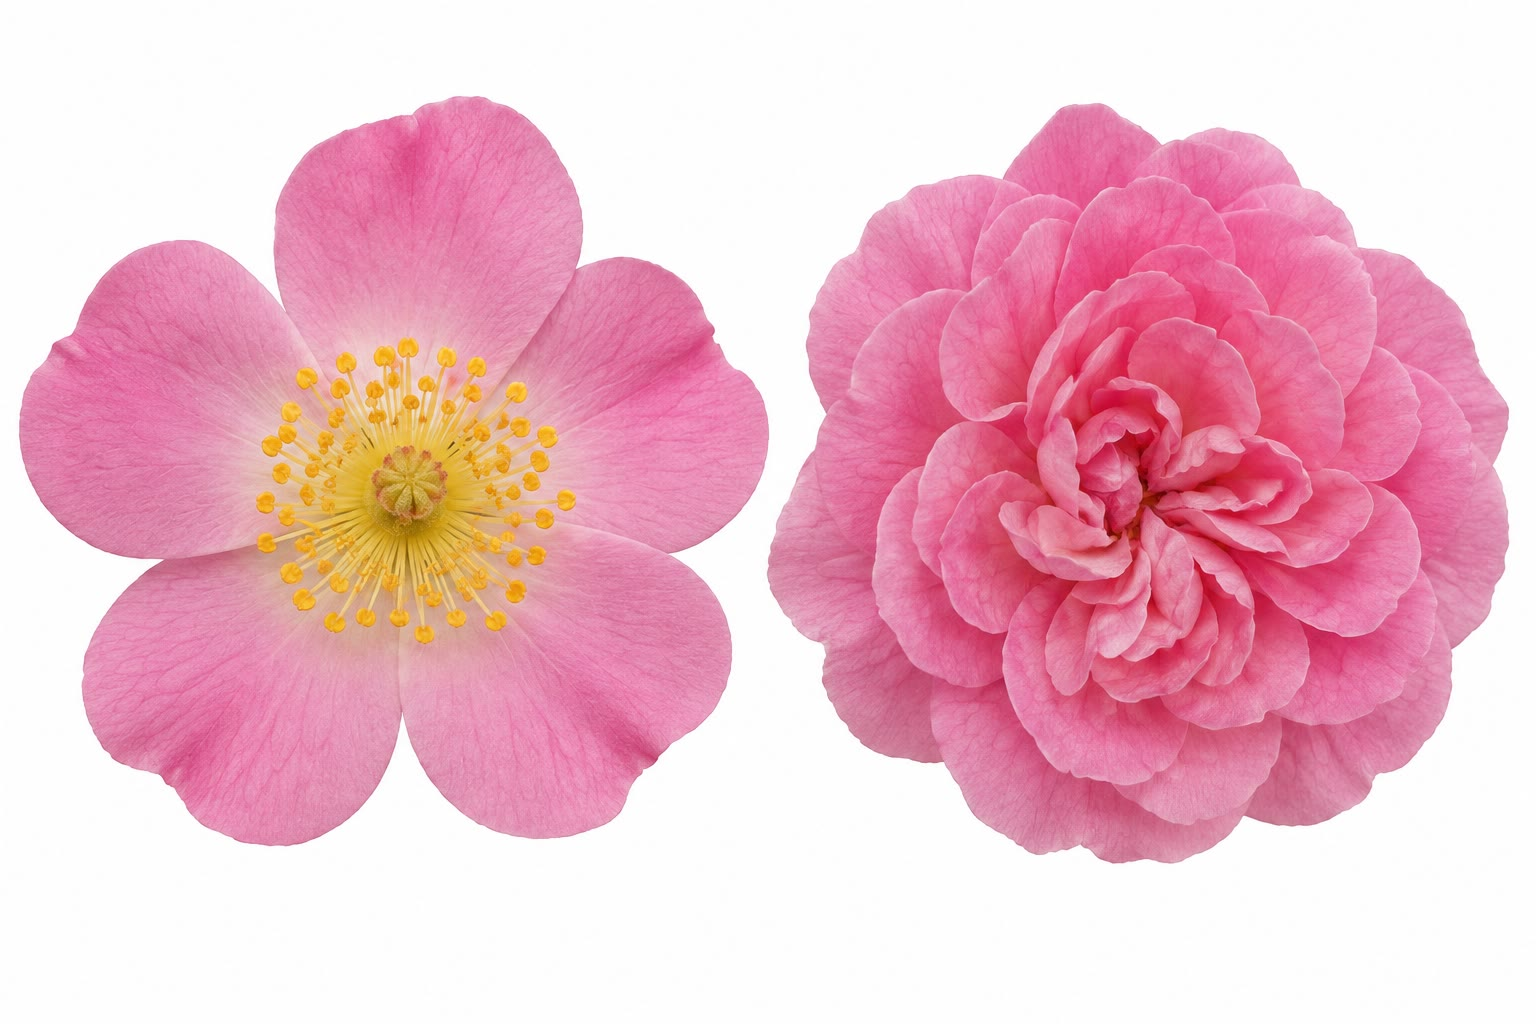
\includegraphics[width=0.58\linewidth]{images/book4/ai/b4-14-double-flower.jpg}

{\small \omterm{def:b2:angiosperm-reproduction:flower}{زهرة} برية بجانب صورة مضاعفة: فقد صارت السدى
بتلات --- أي طافرة في الصنف C، انتخبها البستانيون
قرونًا قبل أن يعرف أحد لماذا كانت مضاعفة.}
\end{omfigure}

\section{السكون والإنبات}

\begin{definition}[سكون البذرة]\label{def:b2:plant-flowering:dormancy}
\index{سكون!البذرة}\index{حمض الأبسيسيك}\index{جبريلين}\index{تطبيق بارد}
\omterm{def:b2:angiosperm-reproduction:seed}{البذرة} الحية التي لا تنبت في ظروف تدعم
النمو \emph{ساكنة}. ويفرض \omterm{def:b2:angiosperm-reproduction:seed}{السكون} خلال نضج \omterm{def:b2:angiosperm-reproduction:seed}{البذرة}
\emph{حمض الأبسيسيك} (ABA)، الذي يقود أيضًا تراكم
المدخرات وتجفيف الجنين، وتصونه \omterm{def:b2:angiosperm-reproduction:seed}{قشرة البذرة}
(غير النفوذة للماء أو للأكسجين، والمقيّدة
ميكانيكيًا) أو حالة الجنين نفسه. ويكسره
الإشارات التي تعلّم نهاية الموسم غير المواتي:
أسابيع من البرد والندى (\emph{التطبيق البارد}، وهو إرباع
\omterm{def:b2:angiosperm-reproduction:seed}{البذرة})، والضوء --- للبذور الصغيرة التي يجب أن تكون قرب
السطح، ويستشعره الفيتوكروم --- أو الظلام، وتناوب
الحرارات، وغسل المثبطات بالمطر، وخدش
القشرة بالتربة أو بأمعاء، والدخان والحرارة بعد حريق. و
القرار توازن بين ABA و\emph{الجبريلين}: فإشارات
الكسر تخفض ABA وترفع الجبريلين الذي يحشد
المدخرات (\cref{ch:b2:angiosperm-reproduction}) ويدع
الجذير ينمو. وجمهرة البذور ليست موحدة: فكسر منها
ينبت عند أول فرصة، وينتظر الباقي سنة أو أكثر،
فلا يقتل موسم رديء واحد الفوجَ كله --- وهو
\emph{بنك البذور}، تحوّط في وجه عالم لا يُتنبأ به.
\end{definition}
\begin{proof}[شواهد]
بذور الخس (بورثويك، 1952) تنبت في الظلام بعد ومضة
من الضوء الأحمر ولا تنبت بعد ومضة من الأحمر البعيد؛ وإذا أُعطيت أحمر ثم
أحمر بعيد ثم أحمر، أنبتت --- فالومضة الأخيرة هي التي تقرر.
والصباغ العكوس نفسه الذي يوقّت الإزهار يبدأ الإنبات.
وبذور أشجار كثيرة مزروعة طازجة في تربة دافئة لا تفعل شيئًا؛ والبذور
نفسها بعد شهرين في برّاد رطب تنبت حالًا،
والطافرات الناقصة ABA تنبت على النبات قبل أن تجف \omterm{def:b2:angiosperm-reproduction:seed}{البذرة}
أصلًا.
\end{proof}

\begin{omfigure}
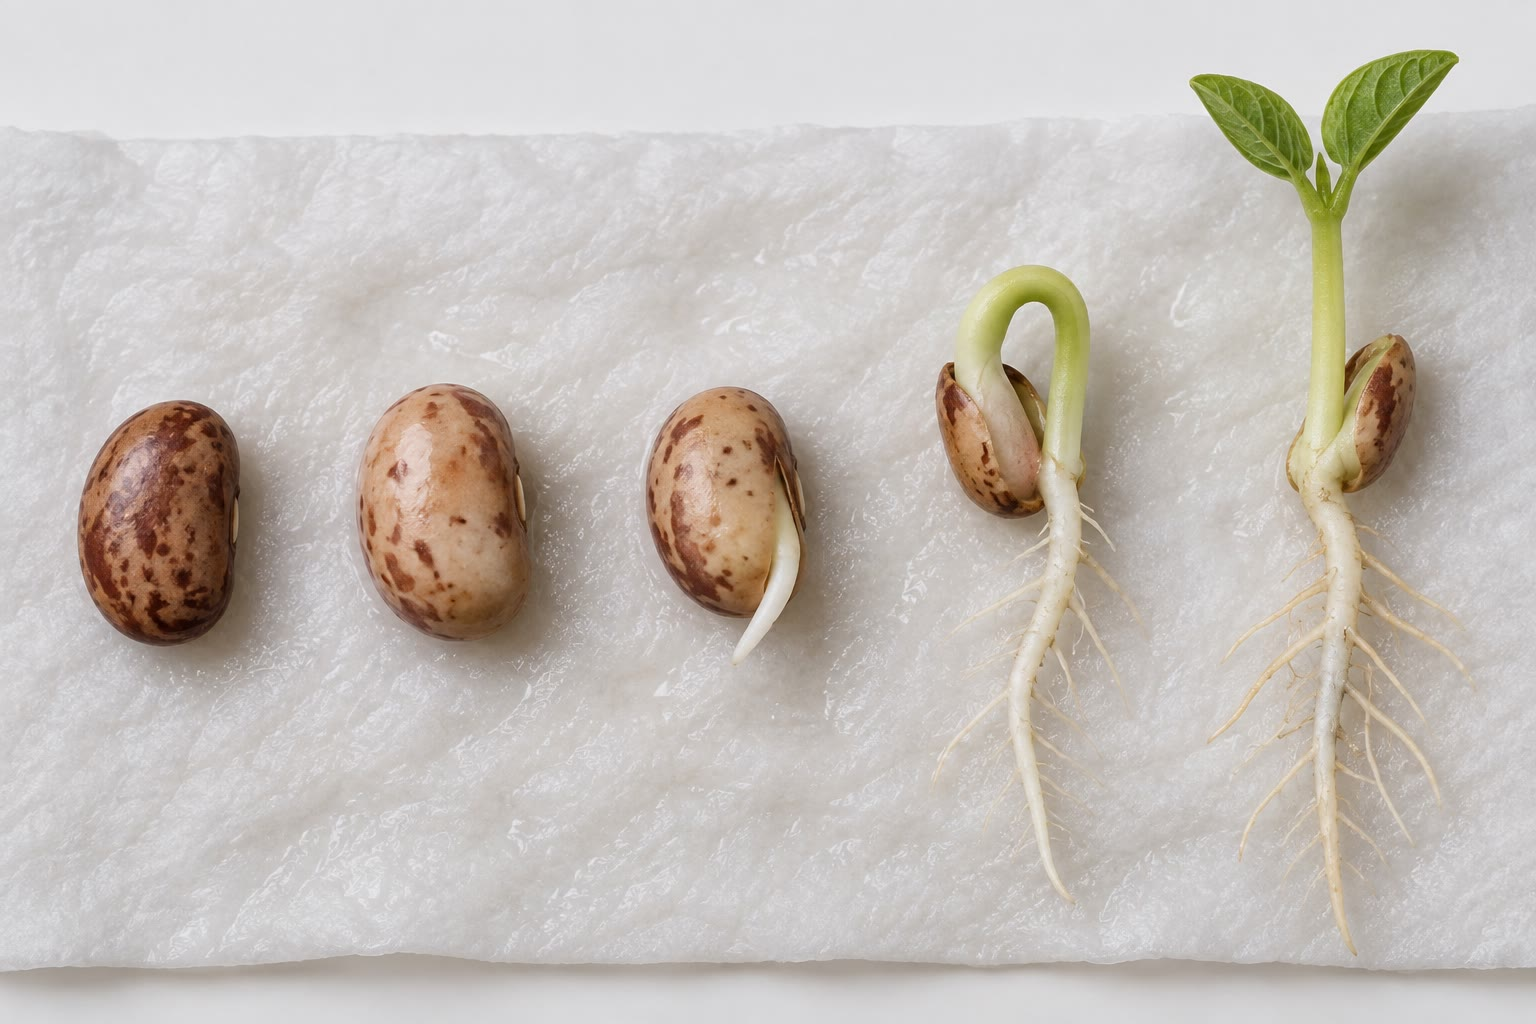
\includegraphics[width=0.66\linewidth]{images/book4/ai/b4-14-germinating-beans.jpg}

{\small إنبات الفاصولياء: تشرب \omterm{def:b2:angiosperm-reproduction:seed}{البذرة}، ويبرز الجذير
أولًا، ويتقوس السويق الجنيني صاعدًا عبر التربة، ويستقيم القوس
في الضوء مع انفتاح الورقتين الأوليين.}
\end{omfigure}

\begin{theorem}[الإنبات رهان]\label{thm:b2:plant-flowering:bet}
\index{تحوّط الرهان}
ليكن كسر $g$ من فوج بذور ينبت كل سنة وينجو
الباقي في التربة باحتمال $s$ إلى السنة التالية. وفي
السنة الجيدة تخلّف \omterm{def:b2:angiosperm-reproduction:seed}{البذرة} المنبتة $R_g$ \omterm{def:b2:angiosperm-reproduction:seed}{بذرة}؛ وفي السنة الرديئة،
لا شيء؛ والسنوات جيدة باحتمال $p$. فالاستراتيجية التي
تنبت كل شيء دفعة واحدة ($g = 1$) لها، على مدى سلسلة من السنوات،
معدل نمو طويل الأمد مأخوذ بمتوسط $\ln$ قدره $p\ln R_g + (1 - p)\ln 0 =
-\infty$: فسنة رديئة واحدة تفنيها. أما الاستراتيجية التي $g < 1$
فتنمو في السنوات الجيدة بعامل $gR_g + (1 - g)s$ وفي السنوات الرديئة
بعامل $(1 - g)s > 0$، فيكون معدلها الطويل الأمد،
\[
r = p\ln\bigl(gR_g + (1 - g)s\bigr) + (1 - p)\ln\bigl((1 - g)s\bigr),
\]
منتهيًا، وهو، من أجل $p$ غير القريبة جدًا من 1، أعظم ما يكون عند
$g$ وسطية. فمع $R_g = 20$، و$s = 0.8$، و$p = 0.7$، يكون
الأمثل قرب $g = 0.7$: أنبت معظمها، وأبقِ احتياطيًا.
\omterm{def:b2:angiosperm-reproduction:seed}{فالسكون} ليس إخفاقًا في الإنبات بل رفضًا جزئيًا
متطوّرًا.
\end{theorem}
\begin{proof}
قياس الجمهرة بعد $T$ سنة جداء العوامل السنوية،
فمعدل نموها متوسط لوغاريتماتها
(أي معدل المتوسط الهندسي)، وهو ما يعظّمه الانتخاب على مدى
الآماد الطويلة. ومع $g = 1$ يكون عامل السنة الرديئة صفرًا واللوغاريتم
$-\infty$. ومن أجل $g < 1$ يكون العاملان موجبين؛ ومفاضلة
$r$ بالنسبة إلى $g$ ووضع المشتق صفرًا يعطيان
الأمثل، وهو من أجل الأرقام المذكورة قرب $g = 0.7$
(فحساب $r$ عند $g = 0.4, 0.6, 0.8, 1$ يعطي $1.28$ و$1.42$
و$1.40$ و$-\infty$).
\end{proof}

\begin{omfigure}
\begin{tikzpicture}
\begin{axis}[
  width=0.7\linewidth, height=5.4cm,
  axis x line=bottom, axis y line=left,
  xmin=0, xmax=1, ymin=0, ymax=1.7,
  xlabel={كسر البذور المنبتة كل سنة، $g$}, ylabel={معدل النمو الطويل الأمد $r$},
  xlabel style={font=\small, at={(axis description cs:0.5,-0.13)}, anchor=north},
  ylabel style={font=\small},
  tick label style={font=\small}, xtick={0,0.2,0.4,0.6,0.8,1}, ytick={0,0.5,1,1.5},
  clip=false,
]
\addplot[very thick, omDef, domain=0.02:0.97, samples=100] {0.7*ln(20*x + 0.8*(1-x)) + 0.3*ln(0.8*(1-x))};
\draw[dashed, gray] (axis cs:0.7,0) -- (axis cs:0.7,1.43);
\node[font=\scriptsize, anchor=south] at (axis cs:0.7,1.45) {الأمثل: أبقِ \qty{30}{\%} في التربة};
\node[font=\scriptsize, anchor=north west, align=left] at (axis cs:0.7,0.6) {$g \to 1$: سنة رديئة واحدة\\تمحو الفوج};
\end{axis}
\end{tikzpicture}

{\small \omterm{thm:b2:plant-flowering:bet}{تحوّط الرهان} \omterm{def:b2:angiosperm-reproduction:seed}{بالسكون}. فمع سنوات جيدة سبعًا من عشر،
يُتلف الفوجَ الذي ينبت كله في النهاية موسمٌ
رديء؛ أما الفوج الذي يبقي حصة من بذوره فينمو أسرع في
الأمد الطويل.}
\end{omfigure}

\section{تمارين}

\begin{exercise}[$\star$]\label{exo:b2:plant-flowering:1}
ميّز المرستيمات الخضرية والنورية والزهرية، وقل
أيها محدد.
\end{exercise}

\begin{exercise}[$\star$]\label{exo:b2:plant-flowering:2}
عرّف النباتات القصيرة النهار والطويلة النهار والمحايدة النهار مع مثال
على كل منها، وقل ماذا يقيس \omterm{prop:b2:plant-flowering:photoperiod}{النبات القصير النهار} فعلًا.
\end{exercise}

\begin{exercise}[$\star$]\label{exo:b2:plant-flowering:3}
أعط هوية العضو في كل دوّارة في النمط البري وفي
الطافرات المفردة الثلاث في \omterm{prop:b2:plant-flowering:abc}{نموذج ABC}.
\end{exercise}

\begin{exercise}[$\star$]\label{exo:b2:plant-flowering:4}
سمِّ أربع إشارات تكسر \omterm{def:b2:angiosperm-reproduction:seed}{سكون} \omterm{def:b2:angiosperm-reproduction:seed}{البذرة}، وسمِّ في كل منها الموسم
أو المكان الذي تبلّغ عنه.
\end{exercise}

\begin{exercise}[$\star\star$]\label{exo:b2:plant-flowering:5}
\omterm{prop:b2:plant-flowering:photoperiod}{نبات قصير النهار} ليله الحرج \qty{10}{h}. قل هل
يزهر تحت: \qty{16}{h} ضوءًا/\qty{8}{h} ظلامًا؛ و\qty{12}{h}/\qty{12}{h}؛ و
\qty{12}{h} ضوءًا و\qty{6}{h} ظلامًا ودقيقة ضوء و\qty{6}{h} ظلامًا؛ و
\qty{8}{h} ضوءًا و\qty{4}{h} ظلامًا و\qty{4}{h} ضوءًا و\qty{8}{h} ظلامًا.
\end{exercise}

\begin{exercise}[$\star\star$]\label{exo:b2:plant-flowering:6}
تُطعَّم ورقة من \omterm{prop:b2:plant-flowering:photoperiod}{نبات قصير النهار} مستحَث على \omterm{prop:b2:plant-flowering:photoperiod}{نبات طويل
النهار} مبقًى في أيام طويلة، فيزهر \omterm{prop:b2:plant-flowering:photoperiod}{النبات الطويل النهار}. فماذا يبين
هذا عن \omterm{def:b2:plant-flowering:florigen}{الفلوريجين}؟ وماذا لو أُجري التطعيم بورقة
مستحَثة لكن لحاؤها مقطوع عند
السويق؟
\end{exercise}

\begin{exercise}[$\star\star$]\label{exo:b2:plant-flowering:7}
يسكت البرد الكابت عند $\alpha = 0.05$ في اليوم و
يحتاج الإزهار إلى $f < 0.15$. فكم يومًا باردًا يلزم؟ و
شتاء فيه ثلاث موجات برد من 15 و12 و20 يومًا يفصل بينها
ذوبان: فهل يُرباع النبات؟ وماذا لو كان $\alpha$ يساوي $0.02$؟
\end{exercise}

\begin{exercise}[$\star\star$]\label{exo:b2:plant-flowering:8}
اشرح لماذا تضيع ذاكرة الإرباع عند النبات في بذوره،
بدلالة الصبغين، ولماذا يكون ذلك مفيدًا.
\end{exercise}

\begin{exercise}[$\star\star$]\label{exo:b2:plant-flowering:9}
تُعطى بذور خس، في الظلام، التعاقبات: أحمر؛ أحمر ثم أحمر بعيد؛
أحمر ثم أحمر بعيد ثم أحمر؛ أحمر ثم أحمر بعيد ثم أحمر ثم أحمر بعيد. تنبّأ بالإنبات في كل حالة و
اشرح بدلالة صورتي الفيتوكروم.
\end{exercise}

\begin{exercise}[$\star\star\star$]\label{exo:b2:plant-flowering:10}
في نموذج \omterm{thm:b2:plant-flowering:bet}{تحوّط الرهان} مع $R_g = 20$، و$s = 0.8$، احسب
معدل النمو الطويل الأمد من أجل $g = 0.4$ و$0.6$ و$0.8$ و$1$ حين
$p = 0.7$، ثم حين $p = 0.95$. وكيف ينزاح الأمثل،
وبماذا يتنبأ ذلك في الصحارى في مقابل المروج؟
\end{exercise}

\begin{exercise}[$\star\star\star$]\label{exo:b2:plant-flowering:11}
تنبّأ \omterm{def:b2:angiosperm-reproduction:flower}{بالزهرة} الناتجة عن التعبير عن مورّثة من الصنف B في الدوّارات
الأربع كلها؛ وعن التعبير عن الصنف C في الأربع كلها؛ وعن طافرة مضاعفة
تفتقر إلى A وB. ثم اشرح لماذا تمضي \omterm{def:b2:angiosperm-reproduction:flower}{الزهرة} الخالية من C في صنع
دوّارات.
\end{exercise}

\begin{exercise}[$\star\star\star$]\label{exo:b2:plant-flowering:12}
«النبات يقرر أن يزهر بمكاملة إشارات لا يستطيع
التحكم فيها.» ناقش المكاملات الثلاث في هذا الفصل --- مكاملة
طول النهار، والبرد، والسنوات في بنك البذور --- وما الذي يحمي
منه المكاملُ النباتَ ولا تحمي منه عتبةٌ بسيطة.
\end{exercise}

\section{مسألة: تقويم المزارع}

\begin{problem}[{مسألة نهاية الأسبوع --- مزارع أقحوان يجدول
الإزهار بالأضواء، ومربّي قمح يعدّ البرد، وزهرة بائع الزهور
المضاعفة تُشرح، وسكون دفعة بذور يُنمذَج،
وتنتهي إلى طول الليل الذي يطلق المحصول، وأيام البرد
التي يحتاجها القمح، وأفضل كسر إنبات}]
\label{pb:b2:plant-flowering:1}
الأقحوان \omterm{prop:b2:plant-flowering:photoperiod}{نبات قصير النهار} طول ليله الحرج
\qty{9.5}{h}؛ ويقتضي الاستحثاث \num{12} ليلة استحثاثية
متتالية، وتتفتح الأزهار بعد \num{8} أسابيع من الاستحثاث. وفي تشرين الثاني
تكون الدفيئة مظلمة من 17:00 إلى 07:30. وقمح الشتاء
له $\alpha = 0.06$ في اليوم البارد ويزهر حين $f < 0.10$. ودفعة
البذور: $R_g = 15$، و$s = 0.7$، والسنوات جيدة باحتمال $p$.

\medskip
\noindent\textbf{الجزء الأول --- الدفيئة.}
\begin{enumerate}
  \item في حزيران يكون الليل الطبيعي \qty{8}{h}. فهل يزهر
        المحصول؟ وماذا على المزارع أن يفعل ليبيع أزهارًا في آب؟
  \item يغطي المزارع المحصول بقماش أسود من
        19:00 إلى 07:00. فأي طول ليل يراه
        النبات، ومتى يجب أن تبدأ التغطية لتفتح في
        15~آب؟
  \item في تشرين الثاني يكون الليل الطبيعي \qty{14}{h} ويريد المزارع
        أن \emph{يؤخر} الإزهار إلى عيد الميلاد. اقترح جدول
        إضاءة واشرح لماذا تكفي ومضة قصيرة.
  \item تُعطى الومضة عند 21:00 بدل 00:00،
        فلا يُمنع الاستحثاث. اشرح ذلك بطول
        الليل الحرج.
  \item في ليلة من الليالي الاثنتي عشرة، يُترك القماش. تنبّأ، و
        قل ماذا كان الخرشوف الشوكي ليفعل.
  \item تُعطى الومضة بضوء أخضر فتخفق؛ وبضوء أحمر
        فتنجح؛ وبأحمر يتبعه أحمر بعيد فتخفق. اشرح.
  \item تُطعَّم ورقة واحدة من نبات مستحَث على نبات
        تحت أيام طويلة. تنبّأ، وقل ماذا يعيّن ذلك.
\end{enumerate}

\medskip
\noindent\textbf{الجزء الثاني --- القمح.}
\begin{enumerate}[resume]
  \item كم يومًا باردًا يحتاج القمح؟
  \item زُرع في تشرين الأول، فنال 10 أيام باردة في تشرين الثاني، وكانون
        أول معتدلًا، و25 في كانون الثاني و12 في شباط. فمتى
        يُرباع؟
  \item زُرع في آذار، فنال 6 أيام باردة. فهل يزهر ذلك
        الصيف؟ وما العاقبة الزراعية؟
  \item طافر يفتقر إلى الكابت. تنبّأ بسلوكه وقل
        لماذا يسمي المربّون أقماحًا كهذه «أقماح الربيع».
  \item اشرح لماذا تنجو ذاكرة البرد من انقسامات
        \omterm{def:b2:plant-meristems:meristem}{المرستيم} خلال الربيع ولا تنجو من \omterm{def:b2:meiosis-heredity:meiosis}{التقسم المنصّف} الذي يصنع
        الجيل التالي.
  \item لماذا يجب أن يُعدّ البرد في \omterm{def:b2:plant-meristems:meristem}{المرستيم} لا في
        الأوراق، بخلاف طول النهار؟
\end{enumerate}

\medskip
\noindent\textbf{الجزء الثالث --- بائع الزهور.}
\begin{enumerate}[resume]
  \item وردة مضاعفة لها بتلات حيث يجب أن تكون السدى و
        بضع بتلات زائدة في المركز. فأي صنف من المورّثات
        أخفق؟ أعط صيغة الدوّارات.
  \item هذا الورد عقيم أبًا \omterm{def:b2:plant-life-cycles:heterospory}{للقاح} لكنه يعقد بذورًا أحيانًا.
        اشرح الأمرين \omterm{prop:b2:plant-flowering:abc}{بنموذج ABC}.
  \item حنك سبع له سدى مكان البتلات وكرابل
        مكان السبلات. فأي صنف أخفق؟
  \item تنبّأ \omterm{def:b2:angiosperm-reproduction:flower}{بزهرة} نبات يُعبَّر فيه عن الصنف C
        في الدوّارة 1 إضافةً إلى دوّاراته العادية.
  \item لماذا أنتجت الطفرات نفسها التحولات نفسها
        في وردة وحنك سبع و\emph{Arabidopsis}، وهي نباتات
        يفصلها مئة مليون سنة؟
  \item في الدوّارة 2 من \omterm{def:b2:angiosperm-reproduction:flower}{زهرة} برية يكون A وB فعالين معًا.
        تنبّأ بالعضو لو كان B وحده فعالًا هناك.
\end{enumerate}

\medskip
\noindent\textbf{الجزء الرابع --- دفعة البذور.}
\begin{enumerate}[resume]
  \item احسب معدل النمو الطويل الأمد $r$ من أجل $g = 0.5$ و$0.7$
        و$0.9$ حين $p = 0.8$.
  \item أي الثلاثة أفضل؟ وماذا يحدث عند $g = 1$؟
  \item أعد الحساب من أجل $p = 0.5$ (أي صحراء). فأي $g$ أفضل الآن؟
  \item يزرع مزارع الدفعة كلها في حقل واحد في سنة جيدة و
        يحصد $R_g$ لكل \omterm{def:b2:angiosperm-reproduction:seed}{بذرة}. اشرح لماذا تختلف استراتيجيته
        عن استراتيجية النبات وماذا عليه أن يفعل ليبقي الصنف
        عبر سنة رديئة.
  \item تحتاج البذور إلى الضوء لتنبت. اشرح المعنى
        التكيفي لذلك عند \omterm{def:b2:angiosperm-reproduction:seed}{بذرة} صغيرة، وتنبّأ بما يفعله الحرث
        ببنك البذور.
  \item اذكر النتيجة: طول الليل الحرج وجدول
        التغطية، وحاجة القمح من البرد، وأفضل $g$ من أجل
        $p = 0.8$ و$p = 0.5$.
\end{enumerate}
\end{problem}
